\section{Practical Part}
\phantomsection

\subsection{Differences and similarities between MSSQL and Oracle}

The control structures have the same logic when comes to determine how the computer responds to certain conditions and parameters. These applies not only to SQL, but to other programming languages as C, C++, Python, Java etc.

In this chapter we will analyze how certain examples  in MSSQL and Oracle. The examples will be written for the database calculatoare.

\begin{itemize}
  \item \textbf{IF Statement}\newline
The first difference is the syntax used for the statement: In Oracles we should use the keyword \textit{THEN} after IF and ends the statement with the keyword \textit{END IF} whereas in MSSQL it is not needed.

The second difference is that in  MSSQL we can use a query as part of a Boolean expression, but in Oracle we can not do this, so instead we can declare a variable that will hold the value of the query and after that operate on it.

\begin{figure}[ht!]
    \centering
	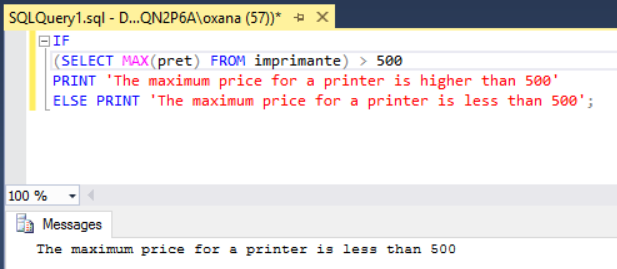
\includegraphics{images/example1-IF.png}
    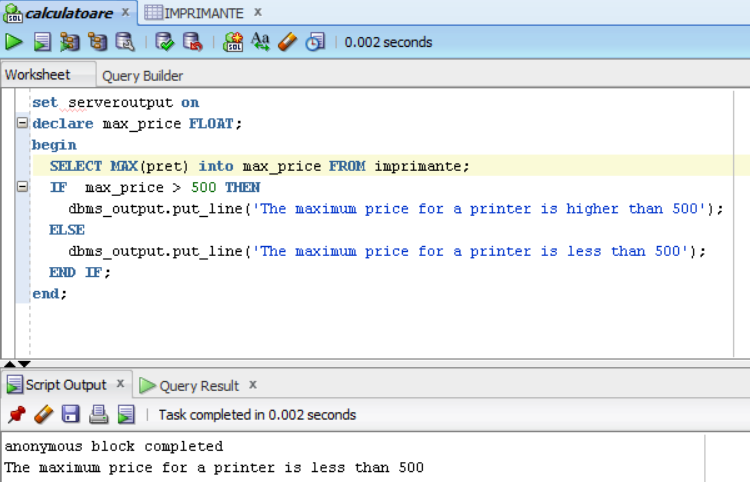
\includegraphics[scale=0.8]{images/example2-IF.png}
    \caption{IF statement in MSSQL and Oracle}
    \label{fig1}
\end{figure}

The maximum price from the printers is 300. So, in this case it is executed the condition after ELSE.

As for the similarities, both MSSQL and Oracle allow nested conditions.

  \item \textbf{CASE Statement}\newline
The difference is that in Oracle if you omit the ELSE clause and none of the search conditions before yields TRUE, than PL/SQL adds the following implicit ELSE clause:
ELSE RAISE CASE\_NOT\_FOUND;

In MSSQL, when this argument is omitted and no comparison operation evaluates to TRUE, CASE returns NULL.

The simmilarity is that in both MSSQL and Oracle can be used searched CASE expressions.

Here is a simple case statement, that compares the selector with the values after WHEN:

\begin{figure}[ht!]
    \centering
    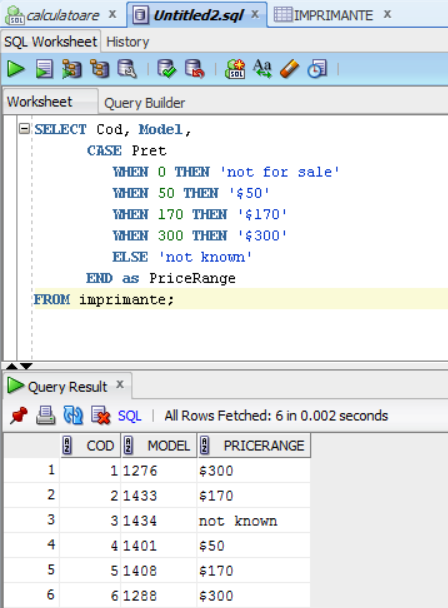
\includegraphics[scale=0.7]{images/example3-case.png}
	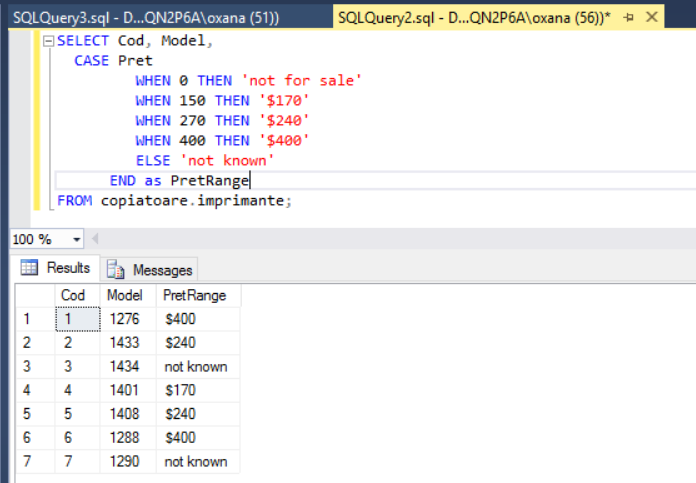
\includegraphics[scale=0.8]{images/example3a-case.png}
    \caption{Case statement in MSSQL and Oracle}
    \label{fig1}
\end{figure}

Now, we can show a searched case, which uses expressions:

\begin{figure}[ht!]
    \centering
	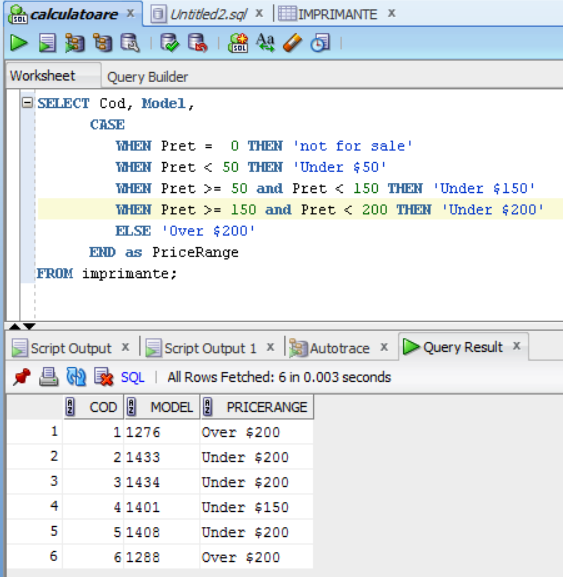
\includegraphics[scale=0.7]{images/example4-searchedcase.png}
    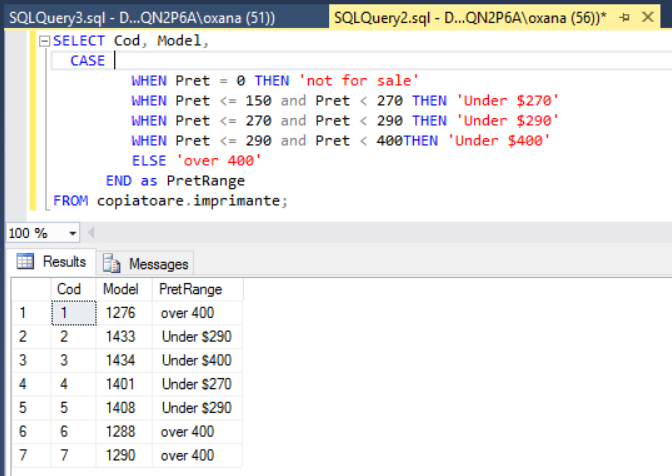
\includegraphics[scale=0.7]{images/example4a-searchedcase.png}
    \caption{Searched case statement in MSSQL and Oracle}
    \label{fig1}
\end{figure}


\item \textbf{Iterative Control}\newline
 The first main difference is that in Oracle we have both WHILE and FOR loops, but in MSSQL there is no FOR loop. In MSSQLWe simulate the FOR LOOP using the WHILE LOOP.

Another difference is that in MSSQL you can exit a while loop with the keyword BREAK, but in Oracle with the keyword EXIT or EXIT-WHEN.


Here is an While loop, that can break or continue using the specified keywords. In the following example, if the average  price of a printer is less than \$300, the WHILE loop doubles the prices and then selects the maximum price. If the maximum price is less than or equal to \$500, the WHILE loop restarts and doubles the prices again. This loop continues doubling the prices until the maximum price is greater than \$500, and then exits the WHILE loop and prints a message.\newline

\begin{figure}[ht!]
    \centering
    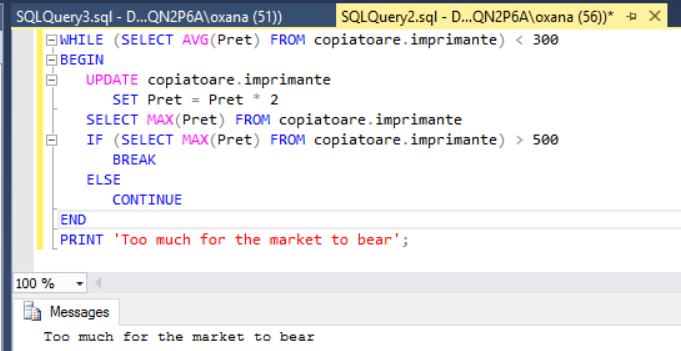
\includegraphics{images/example5-while.png}
    \caption{While loop in MSSQL}
    \label{fig1}
\end{figure}

In Oracle it is also used the LOOP keyword. In the following case the avg\_price will be doubled until it gets bigger than 400.
\begin{figure}[ht!]
    \centering
    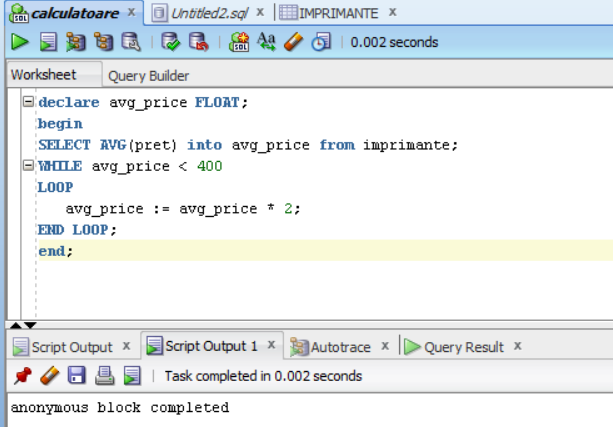
\includegraphics{images/example5-whileloop.png}
    \caption{While loop in Oracle}
    \label{fig1}
\end{figure}\newline


In Oracle, the FOR LOOP allows you to execute code repeatedly for a fixed number of times. This FOR LOOP example will loop 20 times. The counter called i will start at 1 and end at 20. So, it will double the avg\_price 20 times. \newline\newline\newline\newline


 \begin{figure}[ht!]
    \centering
    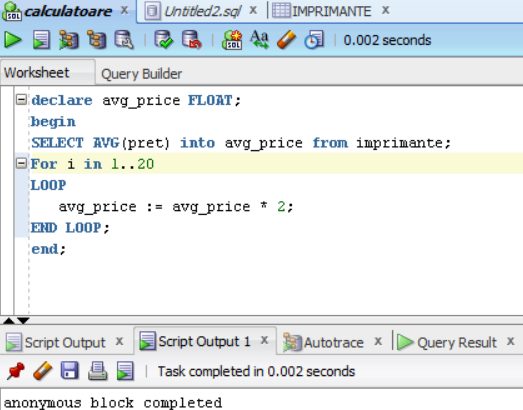
\includegraphics{images/example6-for.png}
    \caption{For loop in Oracle}
    \label{fig1}
\end{figure}

\item \textbf{GOTO}\newline

Both in Oracle and MSSQL use GOTO label to alter the flow of the execution. They have similar implementation, the only difference is that in Oracle the label name is in between $\ll$ and $\gg$.

The following example in MSSQL will jump to the finished label when the maximum price of the printer will exceed 300.

 \begin{figure}[ht!]
    \centering
    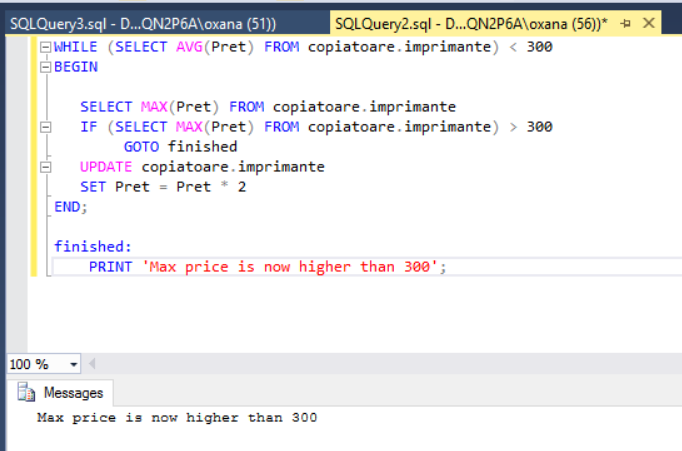
\includegraphics{images/example7-goto.png}
    \caption{GOTO in MSSQL}
    \label{fig1}
\end{figure}


The next example, in Oracle has a while loop that will stop when the max price will be higher than 1000. However, the goto label can interrupt the flow of control and jump to the printing line. So, in this case when the max price gets higher than 500, it will jump to the label finish\_loop.
 \begin{figure}[ht!]
    \centering
    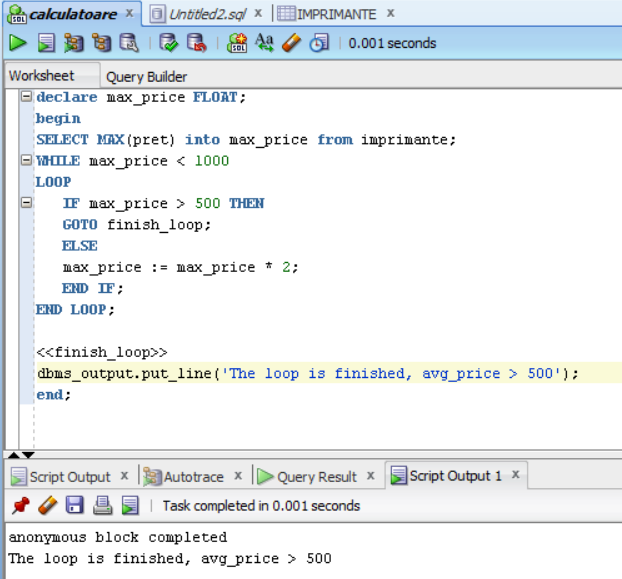
\includegraphics{images/example7a-goto.png}
    \caption{GOTO in Oracle}
    \label{fig1}
\end{figure}


\end{itemize}
\clearpage